\documentclass[border=3mm]{standalone}
\usepackage{tikz}
\usetikzlibrary{positioning,fit,matrix}

\definecolor{mybluei}{RGB}{124,156,205}
\definecolor{myblueii}{RGB}{73,121,193}
\definecolor{mygreen}{RGB}{202,217,126}
\definecolor{mypink}{RGB}{233,198,235}

\newcommand\widernode[5][widebox]{
  \node[
    #1,
    fit={(#2) (#3)},
    label=center:{\sffamily\bfseries\color{white}#4}] (#5) {};
}

\begin{document}

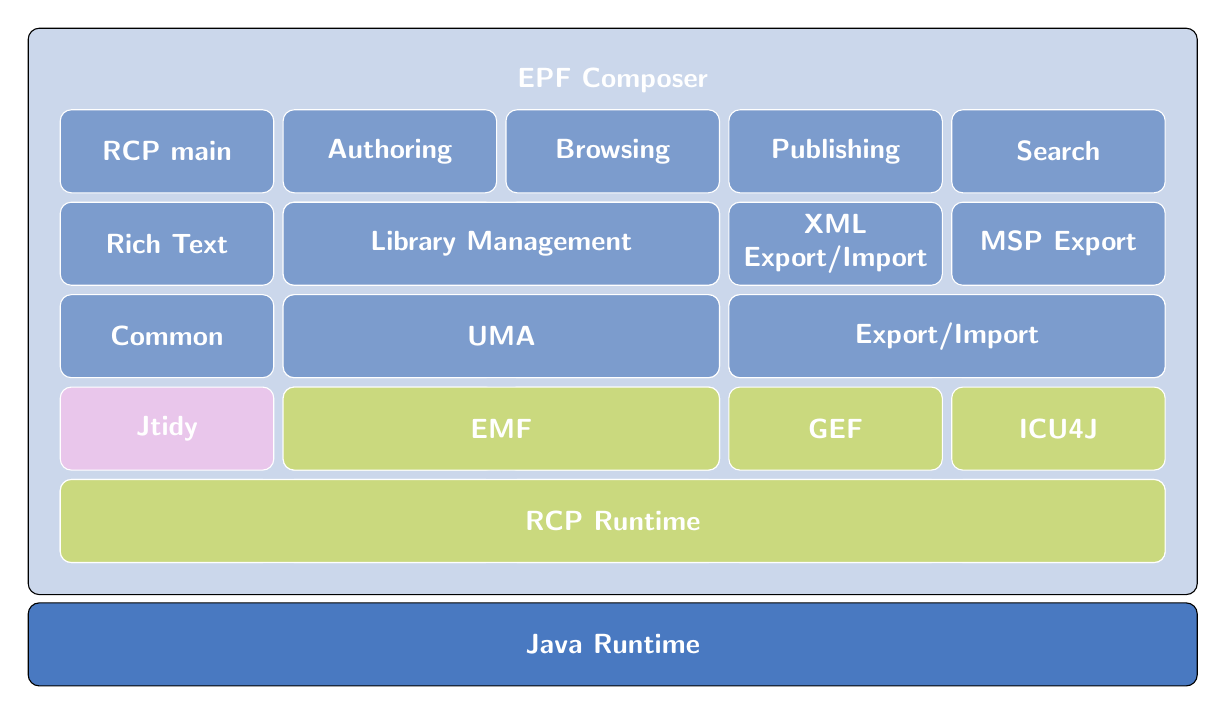
\begin{tikzpicture}[
    node distance=3pt,outer sep=0pt,
    boxstyle/.style={draw=white, fill=#1, rounded corners, font={\sffamily\bfseries\color{white}}, 
                      align=center, minimum height=30pt},
    box/.style={boxstyle=#1,text width=2.5cm},
    box/.default=mybluei,
    title/.style={font={\sffamily\bfseries\color{white}}},
    widebox/.style={draw=white,inner sep=0pt, rounded corners,fill=#1},
    widebox/.default=mybluei,
    mylabel/.style={font={\sffamily\bfseries\color{white}}},]

    \matrix (stack) [boxstyle=mybluei!40, draw=black,%  
                      column sep=3pt, row sep=3pt, inner sep=4mm,%
                      matrix of nodes,% 
                      nodes={box, outer sep=0pt, anchor=center, inner sep=3pt},%  
                      nodes in empty cells, row 1/.style={nodes={fill=none,draw=none,minimum height=3mm}},]
                    {&  & EPF Composer & & \\    
                     RCP main & Authoring & Browsing & Publishing & Search\\    
                     Rich Text & & &{XML\\ Export/Import} & MSP Export\\    
                     Common & & & & \\    
                     |[box=mypink]| Jtidy & & &|[box=mygreen]| GEF &|[box=mygreen]| ICU4J \\    
                     & & & & \\};

    \widernode{stack-3-2}{stack-3-3}{Library Management}{LMg}
    \widernode{stack-4-2}{stack-4-3}{UMA}{UMA}
    \widernode{stack-4-4}{stack-4-5}{Export/Import}{ExImp}
    \widernode[widebox=mygreen]{stack-5-2}{stack-5-3}{EMF}{EMF}
    \widernode[widebox=mygreen]{stack-6-1}{stack-6-5}{RCP Runtime}{RCPrun}

    \node [fit={(stack.south west)(stack.south east)},boxstyle=myblueii,draw=black,inner sep=0pt,below=3pt of stack.south,anchor=north,label={[mylabel]center:Java Runtime}] (JavaR) {};

\end{tikzpicture}

\end{document}